% --- LaTeX Homework Template - S. Venkatraman ---

% --- Set document class and font size ---

\documentclass[letterpaper, 11pt]{article}

% --- Package imports ---

\usepackage{
  amsmath, amsthm, amssymb, mathtools, dsfont,	  % Math typesetting
  graphicx, wrapfig, subfig, float,                  % Figures and graphics formatting
  listings, color, inconsolata, pythonhighlight,     % Code formatting
  fancyhdr, sectsty, hyperref, enumerate, enumitem } % Headers/footers, section fonts, links, lists
  
  \usepackage{tikz}
  \usepackage{amsmath}
\usepackage{amsfonts}
  
  \tikzset{
  vtx/.style={circle, fill=black, inner sep=1.6pt},
  every picture/.style={>=latex}
}

\usetikzlibrary{positioning}

% --- Page layout settings ---

% Set page margins
\usepackage[left=0.7in, right=0.7in, bottom=1in, top=1.1in, headsep=0.2in]{geometry}
\usepackage{tikz}

% Anchor footnotes to the bottom of the page
\usepackage[bottom]{footmisc}



% Set line spacing
\renewcommand{\baselinestretch}{1.2}

% Set spacing between paragraphs
\setlength{\parskip}{1.5mm}

% Allow multi-line equations to break onto the next page
\allowdisplaybreaks

% Enumerated lists: make numbers flush left, with parentheses around them
\setlist[enumerate]{wide=0pt, leftmargin=21pt, labelwidth=0pt, align=left}
\setenumerate[1]{label={(\arabic*)}}

% --- Page formatting settings ---

% Set link colors for labeled items (blue) and citations (red)
\hypersetup{colorlinks=true, linkcolor=blue, citecolor=red}

% Make reference section title font smaller
\renewcommand{\refname}{\large\bf{References}}

% --- Settings for printing computer code ---

% Define colors for green text (comments), grey text (line numbers),
% and green frame around code
\definecolor{greenText}{rgb}{0.5, 0.7, 0.5}
\definecolor{greyText}{rgb}{0.5, 0.5, 0.5}
\definecolor{codeFrame}{rgb}{0.5, 0.7, 0.5}

% Define code settings
\lstdefinestyle{code} {
  frame=single, rulecolor=\color{codeFrame},            % Include a green frame around the code
  numbers=left,                                         % Include line numbers
  numbersep=8pt,                                        % Add space between line numbers and frame
  numberstyle=\tiny\color{greyText},                    % Line number font size (tiny) and color (grey)
  commentstyle=\color{greenText},                       % Put comments in green text
  basicstyle=\linespread{1.1}\ttfamily\footnotesize,    % Set code line spacing
  keywordstyle=\ttfamily\footnotesize,                  % No special formatting for keywords
  showstringspaces=false,                               % No marks for spaces
  xleftmargin=1.95em,                                   % Align code frame with main text
  framexleftmargin=1.6em,                               % Extend frame left margin to include line numbers
  breaklines=true,                                      % Wrap long lines of code
  postbreak=\mbox{\textcolor{greenText}{$\hookrightarrow$}\space} % Mark wrapped lines with an arrow
}

% Set all code listings to be styled with the above settings
\lstset{style=code}

% --- Math/Statistics commands ---

% Add a reference number to a single line of a multi-line equation
% Usage: "\numberthis\label{labelNameHere}" in an align or gather environment
\newcommand\numberthis{\addtocounter{equation}{1}\tag{\theequation}}

% Shortcut for bold text in math mode, e.g. $\b{X}$
\let\b\mathbf

% Shortcut for bold Greek letters, e.g. $\bg{\beta}$
\let\bg\boldsymbol

% Shortcut for calligraphic script, e.g. %\mc{M}$
\let\mc\mathcal

% \mathscr{(letter here)} is sometimes used to denote vector spaces
\usepackage[mathscr]{euscript}

% Convergence: right arrow with optional text on top
% E.g. $\converge[w]$ for weak convergence
\newcommand{\converge}[1][]{\xrightarrow{#1}}

% Normal distribution: arguments are the mean and variance
% E.g. $\normal{\mu}{\sigma}$
\newcommand{\normal}[2]{\mathcal{N}\left(#1,#2\right)}

% Uniform distribution: arguments are the left and right endpoints
% E.g. $\unif{0}{1}$
\newcommand{\unif}[2]{\text{Uniform}(#1,#2)}

% Independent and identically distributed random variables
% E.g. $ X_1,...,X_n \iid \normal{0}{1}$
\newcommand{\iid}{\stackrel{\smash{\text{iid}}}{\sim}}

% Equality: equals sign with optional text on top
% E.g. $X \equals[d] Y$ for equality in distribution
\newcommand{\equals}[1][]{\stackrel{\smash{#1}}{=}}

% Math mode symbols for common sets and spaces. Example usage: $\R$
\newcommand{\R}{\mathbb{R}}   % Real numbers
\newcommand{\C}{\mathbb{C}}   % Complex numbers
\newcommand{\Q}{\mathbb{Q}}   % Rational numbers
\newcommand{\Z}{\mathbb{Z}}   % Integers
\newcommand{\N}{\mathbb{N}}   % Natural numbers
\newcommand{\F}{\mathcal{F}}  % Calligraphic F for a sigma algebra
\newcommand{\El}{\mathcal{L}} % Calligraphic L, e.g. for L^p spaces

% Math mode symbols for probability
\newcommand{\pr}{\mathbb{P}}    % Probability measure
\newcommand{\E}{\mathbb{E}}     % Expectation, e.g. $\E(X)$
\newcommand{\var}{\text{Var}}   % Variance, e.g. $\var(X)$
\newcommand{\cov}{\text{Cov}}   % Covariance, e.g. $\cov(X,Y)$
\newcommand{\corr}{\text{Corr}} % Correlation, e.g. $\corr(X,Y)$
\newcommand{\B}{\mathcal{B}}    % Borel sigma-algebra

% Other miscellaneous symbols
\newcommand{\tth}{\text{th}}	% Non-italicized 'th', e.g. $n^\tth$
\newcommand{\Oh}{\mathcal{O}}	% Big-O notation, e.g. $\O(n)$
\newcommand{\1}{\mathds{1}}	% Indicator function, e.g. $\1_A$

% Additional commands for math mode
\DeclareMathOperator*{\argmax}{argmax}    % Argmax, e.g. $\argmax_{x\in[0,1]} f(x)$
\DeclareMathOperator*{\argmin}{argmin}    % Argmin, e.g. $\argmin_{x\in[0,1]} f(x)$
\DeclareMathOperator*{\spann}{Span}       % Span, e.g. $\spann\{X_1,...,X_n\}$
\DeclareMathOperator*{\bias}{Bias}        % Bias, e.g. $\bias(\hat\theta)$
\DeclareMathOperator*{\ran}{ran}          % Range of an operator, e.g. $\ran(T) 
\DeclareMathOperator*{\dv}{d\!}           % Non-italicized 'with respect to', e.g. $\int f(x) \dv x$
\DeclareMathOperator*{\diag}{diag}        % Diagonal of a matrix, e.g. $\diag(M)$
\DeclareMathOperator*{\trace}{trace}      % Trace of a matrix, e.g. $\trace(M)$

% Numbered theorem, lemma, etc. settings - e.g., a definition, lemma, and theorem appearing in that 
% order in Section 2 will be numbered Definition 2.1, Lemma 2.2, Theorem 2.3. 
% Example usage: \begin{theorem}[Name of theorem] Theorem statement \end{theorem}
\theoremstyle{definition}
\newtheorem{theorem}{Theorem}[section]
\newtheorem{proposition}[theorem]{Proposition}
\newtheorem{lemma}[theorem]{Lemma}
\newtheorem{corollary}[theorem]{Corollary}
\newtheorem{definition}[theorem]{Definition}
\newtheorem{example}[theorem]{Example}
\newtheorem{remark}[theorem]{Remark}

% Un-numbered theorem, lemma, etc. settings
% Example usage: \begin{lemma*}[Name of lemma] Lemma statement \end{lemma*}
\newtheorem*{theorem*}{Theorem}
\newtheorem*{proposition*}{Proposition}
\newtheorem*{lemma*}{Lemma}
\newtheorem*{corollary*}{Corollary}
\newtheorem*{definition*}{Definition}
\newtheorem*{example*}{Example}
\newtheorem*{remark*}{Remark}
\newtheorem*{claim}{Claim}
\newcommand{\Tau}{\mathcal{T}}
\newcommand{\PSet}{\mathcal{P}}





% --- Left/right header text (to appear on every page) ---

% Include a line underneath the header, no footer line
\pagestyle{fancy}
\renewcommand{\footrulewidth}{0pt}
\renewcommand{\headrulewidth}{0.4pt}

% Left header text: course name/assignment number
\lhead{MAM4000W, Graph Theory -- Chapter 6 Problems}

% Right header text: your name
\rhead{Alex Cristaudo, CRSALE010}

% --- Document starts here ---

\begin{document}

\subsection*{Question 1: Find a cubic graph which does not contain a 1-factor}

By Question 2, we need at least 3 bridges. The idea is that our bridges should not be independent, as if they were, our scenario is similar as to if we had 2 bridges.

\begin{figure}[h]
\centering
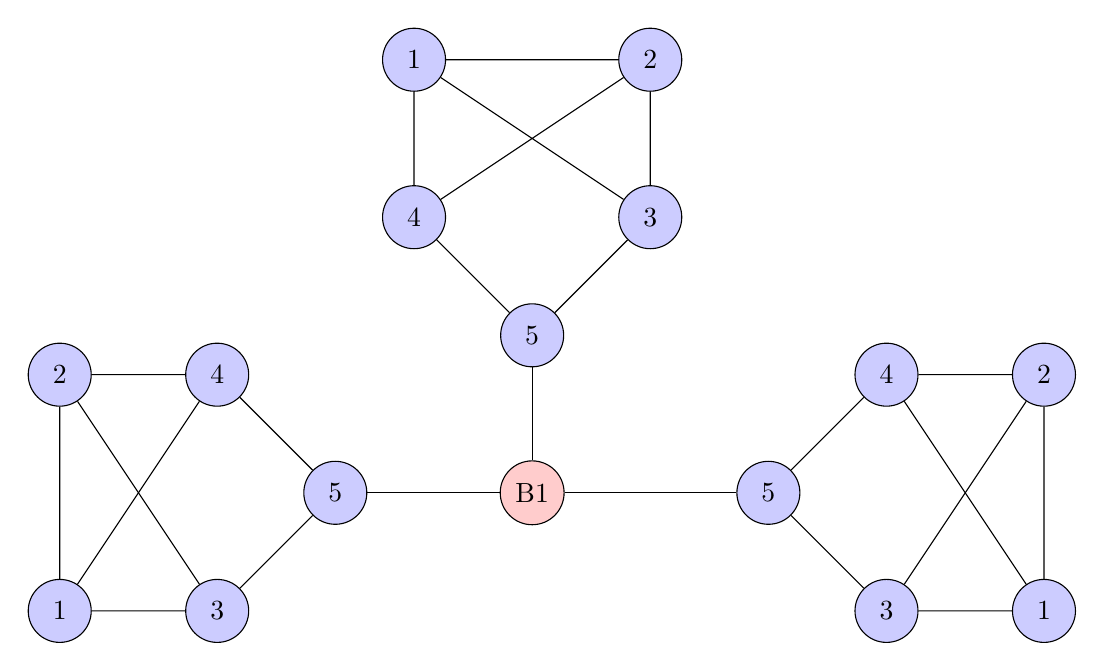
\begin{tikzpicture}[scale=1]
    % Left K_5 vertices
    \node[circle, fill=blue!20, draw, minimum size=8mm] (L1) at (-1,2.5) {1};
    \node[circle, fill=blue!20, draw, minimum size=8mm] (L2) at (2,2.5) {2};
    \node[circle, fill=blue!20, draw, minimum size=8mm] (L3) at (2,0.5) {3};
    \node[circle, fill=blue!20, draw, minimum size=8mm] (L4) at (-1,0.5) {4};
    \node[circle, fill=blue!20, draw, minimum size=8mm] (L5) at (0.5,-1) {5};
    
    \node[circle, fill=red!20, draw, minimum size=8mm] (B1) at (0.5, -3) {B1};
   

    % Right K_5 vertices
    \node[circle, fill=blue!20, draw, minimum size=8mm] (R1) at (7,-4.5) {1};
    \node[circle, fill=blue!20, draw, minimum size=8mm] (R2) at (7,-1.5) {2};
    \node[circle, fill=blue!20, draw, minimum size=8mm] (R3) at (5,-4.5) {3};
    \node[circle, fill=blue!20, draw, minimum size=8mm] (R4) at (5,-1.5) {4};
    \node[circle, fill=blue!20, draw, minimum size=8mm] (R5) at (3.5,-3) {5};

     \node[circle, fill=blue!20, draw, minimum size=8mm] (1) at (-5.5,-4.5) {1};
    \node[circle, fill=blue!20, draw, minimum size=8mm] (2) at (-5.5,-1.5) {2};
    \node[circle, fill=blue!20, draw, minimum size=8mm] (3) at (-3.5,-4.5) {3};
    \node[circle, fill=blue!20, draw, minimum size=8mm] (4) at (-3.5,-1.5) {4};
    \node[circle, fill=blue!20, draw, minimum size=8mm] (5) at (-2,-3) {5};
    
    \draw (L1) -- (L2) -- (L3) -- (L1) -- (L4) -- (L2);
    \draw (L4) -- (L5) -- (L3);
    \draw (B1) -- (L5);


    \draw (1) -- (2) -- (4) -- (5) -- (3) -- (1) -- (4);
    \draw (3) -- (2);
    \draw (5) -- (B1);

    \draw (R1) -- (R2) -- (R4) -- (R5) -- (R3) -- (R1) -- (R4);
    \draw (R3) -- (R2);
    \draw (B1) -- (R5);
    

    
\end{tikzpicture}
\end{figure}
\noindent 
To prove this does not contain a 1-factor, consider removing vertex $B1$. This results in a disconnected graph with 3 odd components, but we removed 1 vertex. Thus Tutte's Theorem tells us that this graph does not contain a 1-factor.

\subsection*{Question 2: Prove that every cubic graph with at most two bridges contains a 1-factor.}
It is sufficient to show that every cubic graph with at most 2 bridges satisfies Tutte's condition. Let $S \subseteq V(G)$ and let $C$ be an odd component of $G - S$. The sum of degree (in $G$) of vertices in $C$ must be odd, since $C$ is cubic. But by the Handshaking Lemma, only an even part of this sum arises from edges contained in $C$. Thus there is an odd sum joining $C$ to $S$ and thus there is an odd number of edges. Now this means, for each odd component $C$, there can be $1$ edge joining $C$ to $S$ (corresponding to a bridge) or at least $3$ edges. Let $r$ be the number of odd components joining to $S$ with only $1$ edge. Then there are at least $3(q(G-S) - r) + r = 3q(G - S) - 2r$ edges from odd components joining $S$. Clearly there are at most $3|S|$ edges joining odd components from $S$. So \[
3q(G - S) - 2r \le 3|S| \Longrightarrow q(G - S) \le |S| + \frac{2}{3}r
\]
Now, $r \le 2$ and $q(G - S)$ and $|S|$ are integers, so we have a stricter inequality:
\[
q(G - S) \le |S| + \frac{4}{3} \Longrightarrow q(G - S) \le |S| + 1
\]
Assume now that $q(G - S) = |S| + 1$. Then from our initial inequality, \[
|S| + 1 \le |S| + \frac{2}{3}r \iff r \ge \frac{3}{2}
\]
Again, $r$ is an integer and so $r = 2$. But then $G$ has $2$ bridges and they join different odd components to $S$. Our lower bound for edges from odd components to $S$ is then $3(|S| + 1) - 4 = 3 |S|-1$. This must then be attained (the other case implies the number of edges is a multiple of 3, but the 2 bridges mean it cannot be), and every other odd component joins $S$ with $3$ edges (as if any odd component joined with more edges, they would be at least $5$ edges and contradict our upper bound). So there is one edge that does not connect $S$ to an odd vertex, and thus either is internal in $S$ or joins to an even component. In both cases, this edge is a bridge which contradicts that $G$ has at most 2 bridges. Thus $q(G - S) = |S| + 1$ is impossible and $q(G - S) \le |S|$, so the Marriage Condition is satisfied.

\subsection*{Question 3: Provide a proof of the Marriage Theorem which utilises Tutte's Theorem.}

\begin{theorem}[Hall's Marriage Theorem]
Let $G = (X, Y, E)$ be a finite bipartite graph with bipartite sets $X$ and $Y$. Then $G$ contains a matching that covers every vertex of $X$ if and only if for every subset $W \subseteq X$, we have
\[
|N_G(W)| \geq |W|,
\]
where $N_G(W)$ denotes the set of all neighbors in $Y$ of vertices in $W$.
\end{theorem}
~\\
Suppose $G$ contains a matching that covers every vertex of $X$. Then the subgraph $H$, induced by $X$, and the set of vertices in $Y$ that are used, contains a perfect matching. But then by Tutte's Theorem, for every $S \subseteq V(H)$, we have $q(H - S) \le |S|$. Let $W \subseteq X$. Then $q(H - N_H(W)) \le |N_H(W)| \le |N_G(W)|$. In $H - N_H(W)$, every vertex in $W$ is isolated (and thus an odd component). Finally, \[|W| \le q(H - N_H(W)) \le |N_G(W)|\]The other direction is proved in Theorem 6.2.4. in the notes.


\subsection*{Question 4: Let $M$ be a sub-optimal matching of a bipartite graph $G$ ($M$ contains less edges than
some other matching of $G$). Prove that $G$ contains an augmenting path with respect
to $M$. Does this fact generalise to non-bipartite graphs? (Hint: use symmetric
difference).}
Let $M$ be a sub-optimal matching, containing less edges than matching $N$. Then the symmetric difference, $M \triangle N = (M - N) \cup (N - M)$ is the edges in either $M$ or $N$, but not both. This is necessarily nonempty because $|N| > |M|$. Now consider the connected components of $G[M \triangle N]$. Every vertex has degree at most $2$ (if they are matched by both $M$ and $N$, less if they are only matched by one). Thus the connected components are either even cycles (alternating edges from $M$ and $N$, equal number from both in each cycle), or paths, possibly with some unmatched endpoints. Since $|N| > |M|$, there must be at least one path component in $M \triangle N$ with more edges from $N$ than from $M$. Such a path, necessarily of odd length, starts and ends at vertices unmatched by $M$ and consists of alternating edges from $N$ and $M$ and is thus an augmenting path for $M$. This fact does generalise to non-bipartite graphs but is complicated (Berge's Theorem)

\subsection*{Question 5: Find an infinite graph which serves as a counter-example to the Marriage Theorem.}
Let $A = \{a_0,a_1,...\}, B = \{b_0, b_1,...\}$ with edges $a_0b_i$ for every $i \in \mathbb{N}_0$, and $a_jb_{j-1}$ for every $j \in \mathbb{N}^+$. We cannot find a matching that covers $X$, as if it did, every edge $a_j b_{j-1}$ must be included, and any edge incident to $a_0$ provides a contradiction. But, for $W \subseteq X$, if $a_0 \notin W$, $|W| = |N_G(W)|$. If $a_0 \in W$, then $|N_G(W)| = \aleph_0 \ge |W|$.

\begin{center}
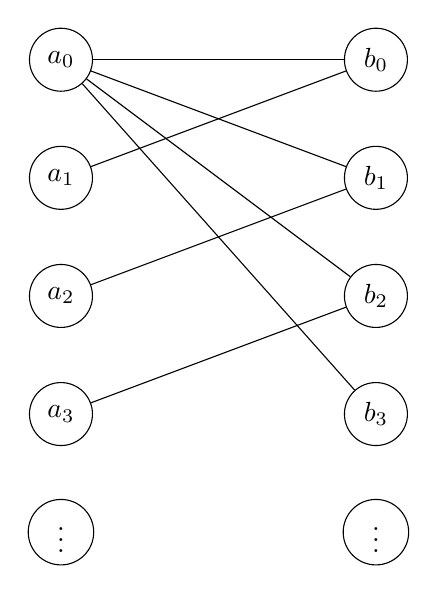
\begin{tikzpicture}[scale=1, every node/.style={circle, draw, minimum size=8mm}]
  % Left set A
  \node (a0) at (0,0) {$a_0$};
  \node (a1) at (0,-1.5) {$a_1$};
  \node (a2) at (0,-3) {$a_2$};
  \node (a3) at (0,-4.5) {$a_3$};
  \node (dotsA) at (0,-6) {$\vdots$};

  % Right set B
  \node (b0) at (4,0) {$b_0$};
  \node (b1) at (4,-1.5) {$b_1$};
  \node (b2) at (4,-3) {$b_2$};
  \node (b3) at (4,-4.5) {$b_3$};
  \node (dotsB) at (4,-6) {$\vdots$};

  % Edges from a0 to all b_i (draw some for example)
  \draw (a0) edge[bend right=0] (b0);
  \draw (a0) edge[bend right=0] (b1);
  \draw (a0) edge[bend right=0] (b2);
  \draw (a0) edge[bend right=0] (b3);

  % Edges a_i to b_{i-1} for i >= 1
  \draw (a1) -- (b0);
  \draw (a2) -- (b1);
  \draw (a3) -- (b2);

\end{tikzpicture}
\end{center}

\subsection*{Question 6: Show that a graph $G$ is bipartite if and only if $\beta (H) \ge \frac{1}{2} |V(H)|$ for every subgraph $H$ of $G$}
Suppose $G$ is bipartite and $H$ is a subgraph of $G$. Let $\{A,B\}$ be a bipartition of $G$. Then $\{A_H, B_H\} := \{A \cap V(H), B \cap V(H)\}$ is a bipartition of $H$, and each set is independent. At least one of these sets must have a size $\ge \frac{1}{2}|V(H)|$, as $V(H) = A_H \cup B_H$. But then $\beta(H) \ge \max \{A_H, B_H\} \ge \frac{1}{2}|V(H)|$. Now suppose that $G$ is not bipartite. Then $G$ contains an odd cycle $H := v_1v_2... v_n v_1$. Then $V(H) = n$. The maximum number of independent vertices is $\frac{n-1}{2} < \frac{1}{2}n$. 

\subsection*{Question 7: Show that every tree has at most one perfect matching}
Let $T$ be a tree and $M_1$ and $M_2$ be 2 distinct perfect matchings of $T$. Let $v_1v_2 \in M_1$ with $v_1v_2 \notin M_2$. Then there must exist an edge incident to $v_2$ in $M_2$. Let this be $v_2v_3$. We cannot have that $v_3 = v_1$. Continuing this process, we get alternating edges $v_3 v_4 \in M_1, v_4v_5 \in M_2, ..., v_kv_{k+1} \in M_1, v_{k+1}v_{k+2} \in M_2$ and so on. If any $v_i = v_j, \quad i \ne j$, this implies the existence of a cycle, which cannot be. Thus the alternating path terminates, which is also a contradiction. Thus every tree has at most one perfect matching.

\subsection*{Question 8: Prove or disprove: A graph $G$ without isolated vertices has a perfect matching if and only if $\alpha ' (G) = \beta ' (G)$}
This is true. First suppose $G$ has a perfect matching $M$. Then $|M| = n/2$ and so $\beta ' (G) = |M| = n/2$ (as a perfect matching is also a maximum matching). But we know that a graph with no isolated vertices satisfies $\alpha ' (G) + \beta ' (G) = n$. So $\alpha ' (G) = n/2 = \beta ' (G)$. On the other hand, suppose $\alpha ' (G) = \beta '(G)$. Again, this implies $\beta ' (G) = n/2$ and we can find a matching $M$ with $n/2$ vertices. This must then be a perfect matching, as each edge is independent and covers $2$ vertices.

\subsection*{Question 9: Show that if $G$ is a bipartite graph without isolated vertices, then $\alpha ' (G) = \beta (G)$}
We know that \begin{align*}
\alpha (G) + \beta (G) & = n \\ 
\alpha ' (G) + \beta ' (G) & = n \\
\alpha (G) & = \beta ' (G)
\end{align*}
(all proven in the notes). This system of inequalities implies $\alpha ' (G) = \beta (G)$.
\end{document}